\section{Site graphs}

\subsection{The category of site-graphs}

Define $\kn = \{A, B,..\}$ a set of agent types, equipped with a site map $\site:\kn\to\nat$.
%Define $\pn$ a set of properties.

\begin{definition}[Site-graphs]
\label{def:site_graphs}
A site-graph is a structure $(\ag,\type,\nodes,\links)$ where
\begin{itemize}
\item $\ag$ is a set of agents, ranged over by $a,b$;
\item $\type:\ag\to \set{A, B,...}$ assigns a type to each agent;
\item $\nodes\subseteq \ag\times\nat\uplus\{\text{free}\}$ is a set of nodes, with a special node free, and where each other node is a pair $(a,i)$ with $a\in\ag$ an agent and $i<\site(\type(a))$ a site of $a$;
\item $\links\subseteq \nodes\times\nodes$ is a set of edges that is \emph{conflict free}: $\forall \xi,\xi'\in\links$, $\xi=\xi'$ or $\xi\cap \xi' \subseteq \{\text{free}\}$.
%\item $p_k\subseteq\nodes$, with $k\in\pn$, is the set of internal states of a site. The pairwise intersection of $\{p_k\}_{k\in\pn}$ is the empty set, that is a site can only have one internal state.
\end{itemize}
Denote $\varepsilon$ the empty $\Sigma$-graph.
\end{definition}

Let us, for convenience, fix a set of agents $\ag$ and the function $\type$ such that for any site graph $G$ we consider $\ag_G\subseteq \ag$.

\begin{definition}[Morphisms on site-graphs]
\label{def:site_morph}
A morphism $h:G\to H$ is a total function on agents $h:\ag_G\to\ag_H$ such that it preserves agent types, nodes, sites and edges:
  \begin{align*}
    &\type(h(a))=\type(a)\\
    &h(u)\in\nodes_H,\text{ for any }u\in\nodes_G\text{ s.t. }
    h(a,i) = (h(a),i) \text{ and }
    h(\text{free})=\text{free}\\
    &h(u,v) = (h(u), h(v))\in\links_H,\text{ for any }u,v\in\nodes_G
  \end{align*}
%and such that it preserves edges: $\xi\in \links_G\implies h(\xi)\in \links_H$, where $h(u,v) = (h(u), h(v))$, for any $$.
%% \item it preserves property sets:
%% \[
%% \set{h(u) : u\in p_{k,G}} \subseteq p_{k,H}, \forall k\in\pn.
%% \]
%% \end{itemize}
\end{definition}
An embedding or a mono, denoted $h:G\lemb H$, is an injective morphism on agents. From agent type and node preservation it follows that a mono is also injective on nodes.

\begin{lemma}
  Site-graphs and their morphisms form a category.
\end{lemma}
\begin{proof}
  The category of site graphs has as objects the site graphs of~\autoref{def:site_graphs} and arrows are the morphisms of~\autoref{def:site_morph}.
%
  Given three site graphs $G_1,G_2,G_3$ and two morphisms $f:G_1\to G_2$, $g:G_2\to G_3$ let $h=f\cdot g$ be the composition of the two. It is defined as follows
  \begin{itemize}
  \item $f\cdot g$ is the composition of $f$ and $g$ on agents;
  \item for $a\in\ag_{G_1}$, $\type(h(a))=g(f(\type(a))$ and we have that $\type(h(a))=h(\type(a))$;
  \item for $(a,i)\in\nodes_{G_2}$, $h(a,i) = g(f(a,i))$ and therefore $h(a,i)=(g(f(a)),i)=(h(a),i)$;
  %\item for any $k\in\pn$, $\{h(u): u\in p_{k,G_1}\}=\{f(g(u)): u\in p_{k,G_1}\}$ and we have that $\{g(v): v\in p_{k,G_2}\}\subseteq p_{k,G_3}$ and $\{f(u): u\in p_{k,G_1}\}\subseteq p_{k,G_2}$, hence $\{h(u): u\in p_{k,G_1}\}\subseteq p_{k,G_3}$.
  \end{itemize}
  If $f$ and $g$ are injective, then so is $h$.
%
  The axioms of associativity and identity law easily hold.
\end{proof}

\begin{definition}[Kappa rules]
  \label{def:rule_site}
  A rule is a span $L\overset{h}{\remb} D \overset{g}{\lemb} R$ such that $h$ and $g$ are monos on site graphs and the following hold
  \begin{itemize}
   %\item for any span $L\overset{h'}{\remb} D' \overset{g'}{\lemb} R$ and any embedding $D\overset{f}{\lemb}D'$ such that $h=h'f$ and $g=g'f$ then $f$ is an isomorphism;
  %\item $\forall a\in\ag_D$, $(a,i)\in\nodes_D\iff (h(a),i)\in\nodes_L \iff (g(a),i)\in\nodes_R$; -it follows from injectivity on nodes
  \item $\forall a\in\ag_D$, $(a,i)\in\nodes_D$ then $[(g(a),i),x] \in\links_R \iff [(h(a),i),y] \in\links_L$;
    %\item if $[(a,i),x] \in\links_R$ and $\nexists b$ such that $h(b)=a$ or $\nexists y$ such that $[(b,i),y]\in\links_D$ then $x\in\sites_R$;
  \item if $a\in\ag_R$ and $a\notin\text{image}(g)$ then $\forall i\in\Sigma_{ag-st}(\type(a))$, $(a,i)\in\nodes_R$ and $\exists \xi\in \links_R$ such that $(a,i)\in \xi$.
  %\item $\forall a\in\ag_D$, $(a,i)\in\nodes_D$ then $(h(a),i)\in p_{k,L}\iff (g(a),i)\in p_{k',R}$.
  \end{itemize}
\end{definition}

The category of site graphs and morphisms does not have all the pushouts. %but does have all pullbacks.

\begin{example}
  Let $a,b$ be two agents with $\type(a)=A$ and $\type(b)=B$.
  Let $G_1$ be the site graph of two linked agents of type $A$ and $B$, and let $G_2$ be the site graph with agent $A$ free.
  \begin{align*}
    G_1 = \big(\{a,b\}; \{(a,1),(b,1)\}; [(a,1),(b,1)]\big)\qquad
    G_2 = \big(\{a\}; \{(a,1)\}; [(a,1),\text{free}] \big)
  \end{align*}
  For the graph $O=\big(\{a\};\{(a,1)\}; \emptyset\big)$ with the obvious morphisms, there is no pushout.
  %  For the two graphs \verb|A(x!1), B(x!1)| and \verb|A(x)| there is no pushout.
\end{example}

However this is not an issue for the dpo rewriting with kappa rules.

\begin{lemma}
  Let $L\overset{h}{\remb} K \overset{g}{\lemb} R$ be a rule and let $M$ and $m:L\emb M$ be a site graph and matching, respectively. The DPO rewriting can be applied whenever the gluing conditions hold.
\end{lemma}
\begin{proof}
  \[
  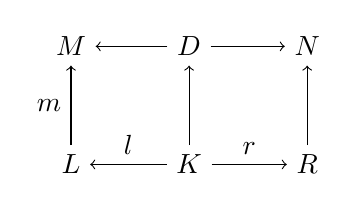
\begin{tikzpicture} %[scale=0.8]
    \node (l) at (-1.5,0) {\(L\)};
    \node (d) at (0,0) {\(K\)};
    \node (r) at (1.5,0) {\(R\)};
    \node (m) at (-1.5,1.5) {\(M\)};
    \node (d') at (0,1.5) {\(D\)};
    \node (n) at (1.5,1.5) {\(N\)};
    \draw [->] (d) -- node [above,midway] {\(l\)} (l);
    \draw [->] (d) -- node [above,midway] {\(r\)} (r);
    \draw [->] (d') -- (m);
    \draw [->] (d') -- (n);
    \draw [->] (l) -- node [left,midway] {\(m\)}  (m);
    \draw [->] (d) -- (d');
    \draw [->] (r) -- (n);
  \end{tikzpicture}
  \]
  We first define a pushout in a "constructive" manner. Then we construct the graph $D$ and show that show that it is a pushout complement. Lastly, we construct $N$ and show that it is the pushout.

  \begin{enumerate}
  \item Let $R\overset{r}{\remb}K\overset{k}{\lemb} D$ be a span and let $N$ be the following graph:
    \begin{itemize}
    \item let $\equiv$ be the smallest equivalence relation with $(k(u),r(u))\in\equiv$, for all $u\in\nodes_K$.
    \item $\nodes_N = (\nodes_D\cup \nodes_R)|_{\equiv}$
    \item $\ag_N = \{a: a\in \text{first}(u), u\in\nodes_N\}$
    \item $\links_N = \{(k(u),k(v)) : (u,v)\in\links_K\}\cup\{(r(u),r(v)) : (u,v)\in\links_R\}$
    %\item $p_{k,N} = k(p_{k,D}) \cup r(p_{k,R})$
    \end{itemize}
    We show that if $N$ is a site graph, i.e. there are no conflicts in $\links_N$ then it is the pushout. Let us suppose that there exists $N'$ and two morphisms $g':D\emb N'$ and $n':R\to N'$ such that $\forall u\in\nodes_K$, $g'(k(u)) = n'(r(u))$. Define the morphism $h:N\to N'$ as follows:
    \begin{align*}
      u\in \nodes_D\cap\nodes_R, &h(u) = g'(k(u)) = n'(r(u))\\
      u\in \nodes_D, u\notin\nodes_R, &h(u) = g'(k(u))\\
      u\in \nodes_R, u\notin\nodes_D, &h(u) = n'(r(u))
    \end{align*}
    The morphism preserves agent types, edges and property sets, which follows from the composition of morphisms. Moreover $h$ is unique.

  \item The graph $D$ is defined as follows:
    \begin{itemize}
    \item $\nodes_D = \nodes_M\setminus m(\nodes_L) \cup m(l(\nodes_K))$
    \item $\links_D = \links_M\setminus m(\links_L) \cup m(l(\links_K))$
    \item $\ag_D = \{a: a\in \text{first}(u), u\in\nodes_D\}$
    %\item $p_{k,D} = p_{k,M}\setminus m(p_{k,L}) \cup m(l(p_{k,K}))$
    \end{itemize}
    It is a site graph, because it is a subgraph of $M$, and therefore there is no conflict on the edges and property sets.

    The morphism $f:D\to M$ is defined as the inclusion morphism.
    Let us now show that $D\overset{f}{\leftarrow}M\overset{g}{\rightarrow} L$ is the pushout of the span $L\overset{l}{\rightarrow}K\overset{k}{\leftarrow} D$. We show that $M$ can be obtained as in the first item of the proof from the graphs $D$ and $L$.

    By manipulating the definition of the set $\nodes_D$ we obtain $\nodes_D\setminus m(l(\nodes_K))\cup m(\nodes_L) = \nodes_M$ which is equivalent to first merging sets $\nodes_D$ and $m(\nodes_L)$ and then define an equivalence class on nodes such that $(m(l(u)),k(u))\in\equiv$, for all $u\in\nodes_K$. Therefore $\nodes_M = (\nodes_D\cup m(\nodes_L))|_{\equiv}$. We proceed similarly for the links. %and the property sets.

  \item The pushout of the span $R\overset{r}{\rightarrow}K\overset{k}{\leftarrow} D$  is constructed as follow:
    \begin{itemize}
    \item let $\equiv$ be the smallest equivalence relation with $(k(u),r(u))\in\equiv$, for all $u\in\nodes_K$.
    \item $\nodes_N = (\nodes_D\cup \nodes_R)|_{\equiv}$
    \item $\ag_D = \{a: a\in \text{first}(u), u\in\nodes_N\}$
    \item $\links_D = \{(k(u),k(v)) : (u,v)\in\links_K\}\cup\{(r(u),r(v)) : (u,v)\in\links_R\}$
    %\item $p_{k,N} = k(p_{k,D}) \cup r(p_{k,R})$
    \end{itemize}
    First let us show that $N$ is a site graph. For that we have to show that $\links_N$ is conflict free. Suppose by contradiction that there exists $[(a,i),(b,j)]\in \links_D$ and $[(a,i),(c,j)]\in \links_R$ and such that $(a,i)\in\nodes_K$. We have then that both $[(a,i),(b,j)]$ and $[(a,i),(c,j)]$ are edges in $N$, which are conflicting.

However, from the definition of rule (\autoref{def:rule_site}), there exists $x$ such that $[(a,i),x]\in\links_L$. As $m:L\lemb M$ is a mono, $[(a,i),x]\in\links_L$ and either $f$ is not a morphism or $x=(b,j)$. But then $[(a,i),x]\in\links_L$ and $r$ is not a morphism. Contradiction.
    %Suppose that there is a conflict in $N$ due to the property sets. For example, let $(a,i)\in p{k,R}$, $(a,i)\in p{k',D}$ and $k\neq k'$. We can reach a contradiction by deriving that $(a,i)\in p{k'',L}$ from \autoref{def:rule_site}.
%
    We have then that $N$ is the pushout from the first item of our proof.
  \end{enumerate}
\end{proof}

\subsection{Influence and dependence in Kappa}

\begin{example}
Let us consider an example, with the following three rules
\begin{verbatim}
  r1: C(y),A(x!1,y),B(x!1)-> C(y!2),A(x!1,y!2),B(x!1)
  r2: A(x!1), B(x!1) -> A(x), B(x)
  r3: C(y!2),A(x,y!2) -> C(y!2),A(x~p,y!2)
\end{verbatim}
Using an inflluence between rules as defined in~\autoref{def:pos_infl} but in the category of site graphs, we get the following influences: $r_2\xrightarrow{+} r_3$ and $r_2\xrightarrow{-} r_1$.
%
There is an influence between $r_1$ and $r_3$ as well, but since there is no pushout for $R_1$ and $L_3$ the definition of influence (\autoref{def:pos_infl}) cannot account for it.
\end{example}

%% \begin{definition}
%%   Define a mapping $\mathcal{F}$ from site graphs to simple graphs
%%   $\mathcal{F}(\ag,\type,\nodes,\links) = (\nodes,\links)$ by forgeting the structure in the nodes.
%% \end{definition}
%% We can show that $\mathcal{F}$ is a functor from the category of site graphs to the one of simple graphs.
%% \begin{definition}
%%   \begin{itemize}
%%   \item Let $G=(V,E)$ be a simple graph, let $\ag$ be a set of agents and let $\ntype:V\to\ag\times\nat\uplus\{\text{free}\}$ be a function that maps nodes in $G$ to pairs \emph{(agent,site)} or to the \emph{free} node. Define $\ntype(G) = (\ag,\nodes,\links)$ as follows:
%%     \begin{align*}
%%       \ag =& \{a: (a,i)\in \ntype(u), u\in V\}\\
%%       \nodes =& \{\ntype(u) : u\in V\}\\
%%       \links =& \{(\ntype(u), \ntype(v)) : u,v\in V\}.
%%     \end{align*}
%%   \item Let $G_1\overset{o_1}{\lemb} O\overset{o_2}{\remb} G_2$ be a span defined on simple graphs such that there exists two functions $\ntype_1$ and $\ntype_2$ with $\ntype_1(G_1)$ and $\ntype_2(G_2)$ site graphs.
%%     We define the following function $\ntype$ on $O$:
%%     \begin{align*}
%%       \ntype(u) =& (a_1,i)\text{ if }\ntype_1(o_1(u))=(a_1,i), \ntype_2(o_2(u))=(a_2,i)\text{ with }\type(a_1)=\type(a_2)\\
%%       & \text{undef, otherwise}
%%     \end{align*}
%%   \end{itemize}
%% \end{definition}
%% We can show that if we take $\ntype$ to be the reverse mapping of $\mathcal{F}$ on nodes, then $\ntype(\mathcal{F}(G))\iso G$.

\begin{definition}[$\Sigma$-graphs]
  A $\Sigma$-graph is a site-graph $(\ag,\nodes,\links)$ where the set of edges is not necessarily conflict free. Morphisms between $\Sigma$ graphs are defined as in~\autoref{def:site_morph}.
\end{definition}
Site-graphs are a full subcategory of the category of $\Sigma$-graph.

%We adapt the influence of~\autoref{def:pos_infl} in the category of $\Sigma$-graphs.

\begin{definition}[Low and medium res influence]
  Let $r_1:L_1{\remb} D_1 {\lemb} R_1$ and $r_2:L_2{\remb} D_2 {\lemb} R_2$ be two rules.
  Let the cospan $R_1\lemb M\remb L_2$ be in the multisum of $R_1$ and $L_2$ in the category of $\Sigma$-graphs. Let the span $\spa:R_1\remb O\lemb L_2$ be its pullback.
  \begin{description}
  \item[low res positive influence]
    There is a \emph{low res positive influence} between the two rules induced by $\spa$ if~\autoref{def:pos_infl} holds and the $\Sigma$-graph $O$ is a site-graph.  We write then $r_1\redl{+}_{\spa} r_2$.
  \item[medium res positive influence]
    There is a \emph{medium res positive influence} between the two rules induced by $\spa$ if there is a low res positive influence and the $\Sigma$-graph $M$ is also a site-graph. We write then $r_1\xrightarrow[med]{+}_{\spa} r_2$.
  \end{description}
\end{definition}
Medium res influence implies a low res influence but not the other way.

The $\Sigma$-graphs are only needed for the definition above. Henceforth, every graphs we consider is a site-graph unless specifically stated otherwise.

%\input{influence_kappa.tex}
The results from~\autoref{sec:ts} hold on site graphs and low res influence. As implied by the example above, the concretisation function will use the low res influence between rules. However, as the pushout of two site graphs is not always a site graphs we have to ensure that whenever we compose transition as in~\autoref{sec:refinement} we do obtain site graphs.

The problem occurs whenever we have two events $e_1$ and $e_2$ for which there is a decoration $R_1\remb O\lemb L_2$ but for which the graph obtained in the pushout is not a site graph. Let us first refine low res precedence to distinguish between the case where the pushout of a decoration yields a site graph and the case where it does not.

\begin{definition}[Dependence on site graphs]
  Let $t_1:M_1\overset{m_1,p_1}{\Rightarrow} N_1$ and $t_2:M_2\overset{m_2,p_2}{\Rightarrow} N_2$ be two transitions in a trace $\theta:t_1;t_1':t_2';\cdots t_n';t_2$ and let $p_1:L_1{\remb} D_1 {\lemb} R_1$ and $p_2:L_2{\remb} D_2 {\lemb} R_2$ be two corresponding rules. The morphism $N_1\pmorph M_2$ is the composition of $\spo(t_1')\circ\dots\spo(t_n')$.
  \begin{description}
%  \item[] $~$
  \item[high res dependence]
    If there exists span $\spa:R_1\remb O\lemb L_2$ such that $p_1\redl{+}_{\spa} p_2$ and for $R_1{\lemb}M{\remb}L_2$ the pushout of $\spa$, the following diagram commutes:
  \[
  \begin{tikzpicture} %[scale=0.8]
    \node (o) at (1,0) {\(O\)};
    \node (m) at (1,2) {\(M\)};
    \node (m1) at (-2,3) {\(M_1\)};
    \node (n1) at (0,3) {\(N_1\)};
    \node (n2) at (4,3) {\(N_2\)};
    \node (m2) at (2,3) {\(M_2\)};
    \node (r1) at (0,1) {\(R_1\)};
    \node (l1) at (-2,1) {\(L_1\)};
    \node (l2) at (2,1) {\(L_2\)};
    \node (r2) at (4,1) {\(R_2\)};
    \draw [->] (o) -- (r1);
    \draw [->] (o) -- (l2);
    \draw [->] (r1) --  (m);
    \draw [->] (r1) --  (n1);
    \draw [->] (l2) --  (m);
    \draw [->] (l2) --  (m2);
    \draw [->] (m) --  (n1);
    \draw [->] (m) --  (m2);
    \draw [-{Stealth[left]}] (n1) --  (m2);
    \draw [->] (l1) --  (m1);
    \draw [->] (r2) --  (n2);
    \draw [vecArrow] (m1) -- node [above,midway] {$m_1,p_1$} (n1);
    \draw [vecArrow] (m2) -- node [above,midway] {$m_2,p_2$} (n2);
    \draw [vecArrow] (l2) -- (r2);
    \draw [vecArrow] (l1) -- (r1);
  \end{tikzpicture}
  \]
  then $t_2$ is high res dependent on $t_1$, denoted $t_1 < t_2$.
\item[medium res dependence]
%  Let $t_1:M_1\overset{m_1,p_1}{\Rightarrow} N_1$ and $t_2:M_2\overset{m_2,p_2}{\Rightarrow} N_2$ be two transitions and let $p_1:L_1{\remb} D_1 {\lemb} R_1$ and $p_2:L_2{\remb} D_2 {\lemb} R_2$ be two corresponding rules.
If there exists $\spa:R_1\remb O\lemb L_2$ such that $p_1\xrightarrow[med]{+}_{\spa} p_2$ and such that the diagram commutes
  \[
  \begin{tikzpicture} %[scale=0.8]
    \node (o) at (1,0) {\(O\)};
    \node (m1) at (-2,3) {\(M_1\)};
    \node (n1) at (0,3) {\(N_1\)};
    \node (n2) at (4,3) {\(N_2\)};
    \node (m2) at (2,3) {\(M_2\)};
    \node (r1) at (0,1) {\(R_1\)};
    \node (l1) at (-2,1) {\(L_1\)};
    \node (l2) at (2,1) {\(L_2\)};
    \node (r2) at (4,1) {\(R_2\)};
    \draw [->] (o) -- (r1);
    \draw [->] (o) -- (l2);
    \draw [->] (r1) --  (n1);
    \draw [->] (l2) --  (m2);
    \draw [-{Stealth[left]}] (n1) --  (m2);
    \draw [->] (l1) --  (m1);
    \draw [->] (r2) --  (n2);
    \draw [vecArrow] (m1) -- node [above,midway] {$m_1,p_1$} (n1);
    \draw [vecArrow] (m2) -- node [above,midway] {$m_2,p_2$} (n2);
    \draw [vecArrow] (l2) -- (r2);
    \draw [vecArrow] (l1) -- (r1);
  \end{tikzpicture}
  \]
  then $t_2$ is medium res dependent on $t_1$, denoted $t_1 \ll t_2$.
  \item[low res dependence]
    If there exists $\spa:R_1\remb O\lemb L_2$ such that $p_1\xrightarrow{+}_{\spa} p_2$ and such that the diagram above commutes, then $t_2$ is low res dependent on $t_1$, denoted $t_1 \prec t_2$.
  \end{description}
\end{definition}

We have that $t_1< t_2 \implies t_1\ll t_2 \implies t_1 \prec t_2$ but not the reverse. As in simple graphs, $\leq$ denotes the transitive and reflexive closure of low res dependence and the causal traces are directed w.r.t. $\leq$. The augmented posets are abstractions of the low res dependence and low res inhibition. %as defined in~\autoref{def:inhibition}.

The following lemma ensures that for any two such events, for which the decoration leads to a conflict in the pushout graph, there exists an event occuring between the two that "resolves" the conflict.

\begin{lemma}
  \label{lem:trace_inhib}
  Let $\theta$ be a causal trace and $t_1:M_1\overset{m_1,p_1}{\Rightarrow} N_1$, $t_2:M_2\overset{m_2,p_2}{\Rightarrow} N_2$ be two transitions such that $t_1\prec t_2$ but $\neg(t_1\ll t_2)$. Then there exists transition $t_3$ such that $t_3\leq t_2$ and either $t_1\prec t_3$ or $t_3\dashv t_1$.
\end{lemma}
\begin{proof}
  Let $\theta':t_1;\cdots t_2$ be a subtrace of $\theta$.
  From $t_1\prec t_2$ and $\neg(t_1\ll t_2)$ we have that there exists $\spa:R_1\leftarrow O\rightarrow L_2$ a span such that $p_1\redl{+}_{\spa} p_2$, but the graph $M$ in the pushout of $\spa$ is not a site graph. It implies that there exists two edges $\xi_1=[(a,i), \text{free}]$ in $R_1$ and $\xi_2=[(a,i),(b,j)]$ in $L_2$ that are in conflict, i.e. the nodes $(a,i)$ in $R_1$ and in $L_2$ map to the same node in $M$. Because of the injective morphisms, we have that $n_1(\xi) \in N_1$ and $m_2(\xi_2)\in M_2$.
  \[
  \begin{tikzpicture} %[scale=0.8]
    \node (o) at (1,0) {\(O\)};
    \node (m) at (1,2) {\(M\)};
    \node (n1) at (0,3) {\(N_1\)};
    \node (m2) at (2,3) {\(M_2\)};
    \node (r1) at (0,1) {\(R_1\)};
    \node (l2) at (2,1) {\(L_2\)};
    \draw [->] (o) -- (r1);
    \draw [->] (o) -- (l2);
    \draw [->] (r1) --  (m);
    \draw [->] (r1) -- node [left,midway] {\(n_1\)} (n1);
    \draw [->] (l2) --  (m);
    \draw [->] (l2) --  node [right,midway] {\(m_2\)} (m2);
    \draw [-{Stealth[left]}] (n1) --  (m2);
  \end{tikzpicture}
  \]
  As $t_2$ is in the trace there exists at least one transition that modifies the edge $m_2(\xi_2)$. Let us consider $t_3$ the earliest such transition in $\theta'$. We first show that $t_3\leq t_2$. By induction on the trace $\theta'$ we look at each transition that modifies the edge for node $(a,i)$. From the kappa rules in~\autoref{def:rule_site} we have that if an edge for $[(a,i),x]\in \links_R$ appears in the right hand side of a rule, then there is an edge that appears in the right hand side $[(a,i),y]\in \links_L$. We deduce therefore a chain of low res dependence between the transitions in $\theta'$ that touch on the edge of node $(a,i)$.

Now let us discuss on the relations between $t_1$ and $t_3$. We distinguish two cases:
\begin{itemize}
\item if $r_1^{-1}(\xi)\in D_1$ and hence node $(a,i)$ is in $L_1$ then we have that $t_3\dashv_{\spa} t_1$ with $\xi_1$ included in the graph $O$ of the span $\spa$;
\item otherwise we have that $t_1\prec_{\spa} t_3$, again with $\xi_1\in O$, where $\spa:R_1\remb O\lemb L_3$.
\end{itemize}
\end{proof}

\begin{remark}[Comparison with asymmetric conflict and inhibition in~\cite{BaldanThesis}]
  In both event structures with asymmetric conflict and inhibition, inhibition in the event structures of~\cite{BaldanThesis} is connected to the causal relation $e_1 < e_2 \implies e_2\dashv e_1$, which is not true in our augmented posets. Moreover, there is no relation in these event structures that can express the different resolutions of dependence.
\end{remark}

\subsection{Interpreting inhibition between kappa posets}
  Let $s_1,s_2$ be two augmented posets and let $(s_1,\theta_1,\mathtt{Ref}_1)$ and $(s_2,\theta_2,\mathtt{Ref}_2)$ be two concretisations for $s_1$ and $s_2$ respectively. Suppose that $\mathtt{Ref}_1(e_1) = M_1\Rightarrow N_1$, $\mathtt{Ref}_2(e_2) = M_2\Rightarrow N_2$ are the two refinements of $e_1$, $e_2$ and $\labl(e_1)\redl{-}_{\spa}\labl(e_2)$, for some cospan $\spa:L_1\remb O\lemb L_2$.
  Whenever $\mathtt{Ref}(e_1\in s_1\redl{-} e_2\in s_2)$ from~\autoref{def:ref_neg_infl} returns the empty set, it implies that the pushout of $M_1$ and $M_2$ is not a site graph. For such cases $\mathtt{Ref}$, instead of returning the empty set, it will return a rule $M_1'\lemb D\remb M_2'$, that intuitively, serves at resolving the conflict in the pushout. If a fictive event produced by this rule, is added as an event to $s_1$ just before $e_1$, then the inhibition between the two events is realised.

\begin{lemma}
  \label{lem:inhibit_site}
  Let $M_1$, $M_2$ be two site-graphs and $M_1\remb O\lemb M_2$ a span, with $M_1\remb M\lemb M_2$ its pushout.
  \begin{itemize}
  \item
  %Let $M$ a $\Sigma$-graph and $M_1$ a site graph such that $M_1\emb M$.
  There exists $N_1$ a site-graph such that the following diagram commutes:
  \[
  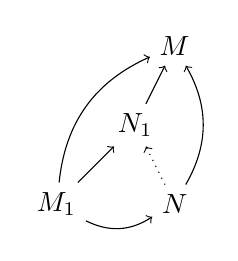
\begin{tikzpicture} %[scale=0.8]
    \node (m) at (1,2) {\(M\)};
    \node (m1) at (-0.5,0) {\(M_1\)};
    \node (n1) at (0.5,1) {\(N_1\)};
    \node (n) at (1,0) {\(N\)};
    \draw [->] (m1) to [bend left] (m);
    \draw [->] (m1) -- (n1);
    \draw [->] (n1) -- (m);
    \draw [->] (n) to [bend right] (m);
    \draw [->] (m1) to [bend right] (n);
    \draw [dotted,->] (n) -- (n1);
  \end{tikzpicture}
  \]
  and such that for any other site-graph $N$ for which the diagram commutes, there exists a unique mono $N\lemb N_1$ that commutes.
  \item Given $N_1$ and $N_2$ constructed as above, there exists a graph $D$ such that $N_1\lemb D\remb N_2$ is a kappa rule.
  \[
  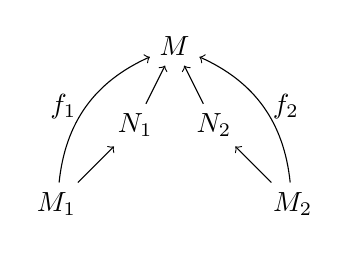
\begin{tikzpicture} %[scale=0.8]
    \node (m) at (1,2) {\(M\)};
    \node (m1) at (-0.5,0) {\(M_1\)};
    \node (n1) at (0.5,1) {\(N_1\)};
    \node (m2) at (2.5,0) {\(M_2\)};
    \node (n2) at (1.5,1) {\(N_2\)};
    \draw [->] (m1) to [bend left] node [left,midway]  {\(f_1\)} (m);
    \draw [->] (m1) -- (n1);
    \draw [->] (n1) -- (m);
    \draw [->] (m2) to [bend right] node [right,midway]  {\(f_2\)} (m);
    \draw [->] (m2) -- (n2);
    \draw [->] (n2) -- (m);
  \end{tikzpicture}
  \]
  \end{itemize}
\end{lemma}
\begin{proof}
  \begin{itemize}
  \item If $M$ is a site-graph then we take $N_1=M$ which satisfies the property. Otherwise, $M$ is not a site graph and therefore there exists $[(a,i),x]$ and $[(a,i),y]$ two conflicting edges in $M$. As $M$ is obtained by pushout of two site graphs we have that either $[(a,i),x]$ or $[(a,i),y]$ is an edge in $M_1$.

    We construct $N_1 = (\ag_1,\nodes_1,\links_1)$ as the site graph $M$ from which whenever there is a pair of conflicting edges, we remove the one that comes from $M_2$:
    \begin{align*}
      \ag_1 = \ag_M\qquad
      \nodes_1 = \nodes_M\qquad
      \links_1 = \links_M\setminus \{ \xi: \exists\xi', \xi\cap \xi'\notin\{\text{free}\}, \xi\in\text{image}(f_2) \}
    \end{align*}
    We have that $N_1$ is a site-graph as there can only be pairs of conflicting edges. Once one of the two is removed, the set of edges is conflict free. The morphism $N_1\lemb M$ is the inclusion on agents and nodes. The morphism $M_1\lemb N_1$ is identical to the morphism $f_1:M_1\lemb M$ as $N_1\subseteq\text{image}(f_1)(M_1)$. Remains to show that for any other site-graph $N$ for which the diagram commutes, there is a unique morphism $h:N\lemb N_1$.
    Let us denote the morphisms as follows: $M_1\overset{g_1}{\lemb}N_1\overset{h_1}{\lemb} M$ and $M_1\overset{g_1'}{\lemb}N\overset{h_1'}{\lemb} M$.
    We define $h$ as follows:
    \begin{align*}
      h(n) = n_1&\text{ if }n\in\text{image}(g_1')\text{ with }m_1\in M_1,g_1'(m_1) = n_1\text{ and }g_1(m_1)=n_1\\
      &\text{ if }n\notin\text{image}(g_1')\text{ then }h_1'(n)=m\in\text{image}(f_2)\text{ and }n_1\in N_1,h_1(n_1) = m
    \end{align*}
    The implication $n\notin\text{image}(g_1')\implies h_1'(n)=m\in\text{image}(f_2)$ follows from $M$ being obtained by pushout. By construction of $N_1$, there exists $n_1\in N_1$ such that $h_1(n_1) = m$. The function is well defined and unique. Indeed, for nodes in $\text{image}(g_1')$ it is straightforward that $h$ is unique. Suppose by contradiction, that there exists $n_1, n_2 \in \text{image}(g_1(N_1))$ such that $h_1(n_1)=h_1(n_2)$. But this contradicts the fact that $h_1$ is an injective morphism.

  \item Define $D=(\ag_D,\nodes_D,\links_D)$ from graph $M$ by removing all pairs of conflicting edges:
    \begin{align*}
      \ag_1 = \ag_M\qquad
      \nodes_1 = \nodes_M\qquad
      \links_1 = \links_M\setminus \{ \xi: \exists\xi', \xi\cap \xi'\notin\{\text{\text{free}}\} \}
    \end{align*}
    The morphisms $D\lemb M_1$ and $D\lemb M_2$ are the inclusions. The constraints of~\autoref{def:rule_site} hold in a straightforward manner.
  \end{itemize}
\end{proof}
